\documentclass{scrartcl}

\usepackage[backend=biber,natbib,style=apa]{biblatex}
\addbibresource{references.bib}

\usepackage[T1]{fontenc}
\usepackage{url}
\usepackage{hyperref}
\usepackage{graphicx}
\usepackage{longtable}
\usepackage{color}
\usepackage{soul}

\DeclareRobustCommand{\hlcyan}[1]{\sethlcolor{cyan}\hl{#1}}
\DeclareRobustCommand{\hlcyan}[1]{#1}

\title{lT2216 Assignment 1: Project proposal}
\subtitle{Investigating move reference in the game of go}
\author{Bill Noble}
\date{\today}

\begin{document}

\maketitle

\section{Background: What is go?}\label{background}

Go\footnote{%
In English, go is also known as 
\emph{baduk} (from Korean),
\emph{weiqi} (from Chinese), or
\emph{igo} (from Japanese).
}%
is an ancient abstract strategy board game for two players.
Worldwide, more people play go than any other board game,
though it is most popular in East Asia.

The board consists of grid intersections. 
A \emph{move} consists of placing a stone on one of the available
intersections.
Players alternate turns, placing stones of their color (black or white).
Points are secured by \emph{capturing}
opponent's stones (by completely surrounding an orthogonally connected \emph{group})
and securing \emph{territory} (a region of empty intersections in which
the opponent cannot possibly play without being captured).
When a group is captured,
the stones are removed from the board and play continues.

There are a few more details (the \emph{rule of ko}, for example),
but from this basic rule set, 
enormous strategic complexity emerges.
On the basis of that complexity, 
a distinct culture of go-playing 
has emerged over its more than 2\,500 year history. 

\begin{figure}[h]
  \centering
  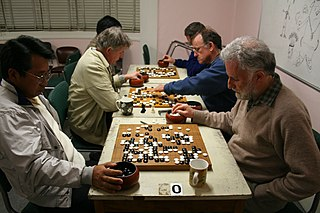
\includegraphics[width=0.6\linewidth]{320px-Go_game_(1907214193).jpg}
  \caption{People playing at a go club in Auckland, New Zealand. Photo: \url{https://commons.wikimedia.org/wiki/File:Go_game_(1907214193).jpg}}
\end{figure}

This project focuses on two aspects of go culture:
\textbf{modes of interaction} 
(ways interacting in the presence of a go board), and
\textbf{move reference}
(ways of talking about different possible next moves).

\section{Modes of interaction}

A \emph{mode of interaction} is related to the idea of a
language game \citep{wittgensteinPhilosophischeUntersuchungenPhilosophical2009}, or
conversational genre \citep{bakhtinSpeechGenresOther1987}.
Although the rules of go specify what game-moves are available to a player
and how to compute the game-effect of a particular game-move
(if the move results in capturing opposing stones, for example),
there are many things about a real-world go-playing interaction that are left
underspecified.
Moreover, there are established ways of interacting
that do not involve playing a game of go \textit{per se},
but that nevertheless 
use knowledge of the rules and shared access to a board
as interactive resources.

\paragraph{competitive play} All of the modes of interaction 
identified here are themselves underspecified in the sense that there 
are additional commonly-understood parameters that affect exactly what kind
of interaction is to take place.
Competitive play is perhaps the most notable example of this.
Competitive games take place on a spectrum from casual to formal.
The most formal competitive games (tournament games, for example),
may explicitly specify additional interaction rules,
such as the use of turn clocks, 
how to take breaks, and
procedures for resolving disputes between players.
In more casual settings (club games, for example),
there are fewer formalized rules around the interaction.
Depending on the conventions of the particular community,
it may be acceptable to have side conversations, 
or even to comment on the game as it is played.

If one of the two players is known to be stronger,
the players may agree to a \textbf{handicap game},
in which some number of the weaker player's stones are placed on the board 
in a particular pattern before play begins.

Other forms of competitive play riff on the two-player paradigm.
In \textbf{simultaneous go}, one (usually stronger) players plays
games against multiple opponents simultaneously.
In \textbf{rengo}, the game is played by two teams of two or more players each.
Players take turns making moves for their team.
In rengo, strategic discussion is typically not allowed within a team, 
but here too different levels of formality may affect what actions are 
considered acceptable.

\paragraph{teaching game} The English-language go wiki 
\textit{Sensei's Library}
describes a teaching game this way:%
\footnote{\url{https://senseis.xmp.net/?TeachingGame}}
\begin{quote}
  A teaching game is a game in which the stronger player teaches the weaker player. Usually their relationship is one of teacher (sensei) and pupil (deshi). The game can be played with full, reduced, or no handicap. The pupil may or may not retake his move. The teacher may or may not give hints as to where to play. The teacher will usually play so as to create instructive situations on the board. The game may or may not be terminated before it is completed. 
\end{quote}

\noindent The article goes on to mention that teaching games may
be provided to a student by a teacher as a paid service.
Here again, the teaching game is a known quantity in the go world,
but the exact parameters of the interaction still 
give room for variation. 

\paragraph{game review} For those who want to improve at go,
game reviews are a way of learning from past games\,---\,%
either one's own or another player's.
A player can review a game solo, 
but game reviews also offer a mode of interaction.
This mode of interaction is different from competitive play and
teaching games because the flow of interaction is not so guided
by the rules of the game itself, though they do 

One typical context for a game review is immediately after 
competitive play. 
One of the players will ask \textit{would you like to review}?
If the other player accepts, 
the two players will typically re-play the game from scratch.
Sometimes one or both of the players will have kept a record,
but often reconstructing the game from memory is part of the 
joint project.
The players will comment on key moves, 
discuss what they were thinking,
and sometimes play out counterfactual variations.
The norms for this mode of interaction are
a subject of discussion in the community.
For example, \textit{Senseis Library}\footnote{https://senseis.xmp.net/?GameReview}
makes the following recommendation:
\begin{quote}
   Use "Black" and "White" instead of naming the players or using pronouns. This creates an objective discussion which allows both players to learn without their ego getting in the way. 
\end{quote}

Another type of game review is when a stronger player 
reviews a game with one or both of its players. 
This is common at tournaments and in club play where 
players of various strengths are present.
Like teaching games, game reviews can also be a mode
of interaction in a student-teacher relationship,
and may be provided in exchange for money.

Since the rise of go-playing AI systems, 
it is common to use AI to help review a game,
especially when reviewing solo.
Players can what moves an AI system would have made in a given situation.
However, the raw output can be difficult to interpret.
Why did the system prefer one move over another?
Programs like \textit{KataGo}, \textit{Leela}, and \textit{AI Sensei}
attempt to improve expandability by visualizing different
possible moves and pre-computing the result of short 
follow-up sequences.

Even with these purpose-built programs,
the AI is not engaging in the kind of   
interaction that you would see in a student-teacher
review or in a review between two players who just finished a game.
One eventual goal of this line of work might be to develop
a system that combines a strong go AI with a dialogue system
to interact in that mode.

\paragraph{other modes} There are of course many other
go-based modes of interaction.
If one attends a go tournament or meeting of a go club,
there might be a \textbf{lecture}, 
where a strong player discusses a particular aspect of the game,
sometimes using a large magnetic \emph{teaching board} 
as a communicative resource.
Game \textbf{commentary} takes many forms.
Like with sports, broadcasts of professional sports games
are usually accompanied by expert commentary.
Written go commentaries have been published in newspapers
and magazines for even longer than broadcast media has existed.
The go \textbf{stream} is a new form of interaction,
similar to a video game stream,
in which a player uses a streaming service like Twitch to live-broadcast 
their competitive play against against other people on the internet.
The streamer will usually comment on the game as it is played,
and viewers can interact with the streamer and each other through text chat.

\section{Move reference}

As in many \emph{communities of practice} \citep{gumperzSpeechCommunity1972},
go-playing communities have special lexicons of \emph{jargon} 
for referring to game-specific concepts. 
In many western go-playing communities 
(certainly in English and Swedish-speaking communities), 
some of these terms are borrowed from Japanese.

Such jargon appears in many different situations.
A board positions might be described as \textit{dangerous for black}.
Taking the other perspective, one might say that 
\textit{whit has good aji} (roughly: potential).
Some players are known to prefer a \textit{fighting game},
while others are more \textit{passive} and prefer to \textit{build}.
In this project, we are interested in how one can refer to 
potential next moves.
This kind of reference is common in several different modes of interaction,
perhaps most notably in game review, 
but also in streaming and commentary and 
perhaps even in 
casual competitive play and teaching games.
In this excerpt from a go stream, I have yellow-highlighted expressions that I think
are referring to potential next moves:\footnote{%
  Technically this was a pre-recorded video (no interaction with the chat), 
  but the live self-commentary format is one used by many streamers.
  Clip here: \url{https://youtu.be/c2sOdbxVtUA?t=247}}

\begin{longtable}{rl}
 1 & Let’s see what he wants to do.\\
 2 &[Black plays R7]\\
 3 &Ah, he’s playing very \emph{very} close \hlcyan{here}.\\
 4 &That’s a bit too close, so let’s do \hl{\textbf{this attachment}} that I mentioned before \\
     & and see what he wants to do.\\
 5 &[White plays P3]\\
 6 &[Black plays P2]\\
 7 & Ahh I can play \hl{\textbf{this}} [gesture: small circle around Q3] to complete my shape \\
 8 &[White plays Q4]\\
 9 &[Black plays R3]\\
10 & And just \hl{\textbf{extend out}}. \\
11 &[White plays O3]\\
12 &And now I have a (..) [gesture: medium circle around P4] really nice shape \\
     & here as white.\\
12 &[Black plays O2]\\
13 &Hmm (..) I think I’m fine with just \hl{\textbf{extending}} still\\
14 &[White plays N3]\\
15 &[Black plays R10]\\
16 &And there we go, he took his (..) \hlcyan{extension} [getsure: line back and forth R7-R10] \\
   & \hlcyan{a little two-space}.\\
17 & I could probably still leave it if I really wanted to [laughs]\\
     & but this could be a good time to try to make the group strong.\\
18 & You could play \hl{\textbf{R16 here to get a base}} [gesure: medium circle around R14]\\
   & which if you play \hl{\textbf{S16}} you’re basically alive after that. \\
19 & You could \hl{\textbf{attach here}} [gesture: hover R11] to get something.\\
20 & Or you could just \hl{\textbf{jump out}} [gesture: hover O14] (...)\\
     & since it feels like there are so many different options (...)\\
     & you probably still don't really need to do anything here \\
     & [gesture: large circle around Q14]\\
\end{longtable}

\begin{figure}[ht]
  \centering
  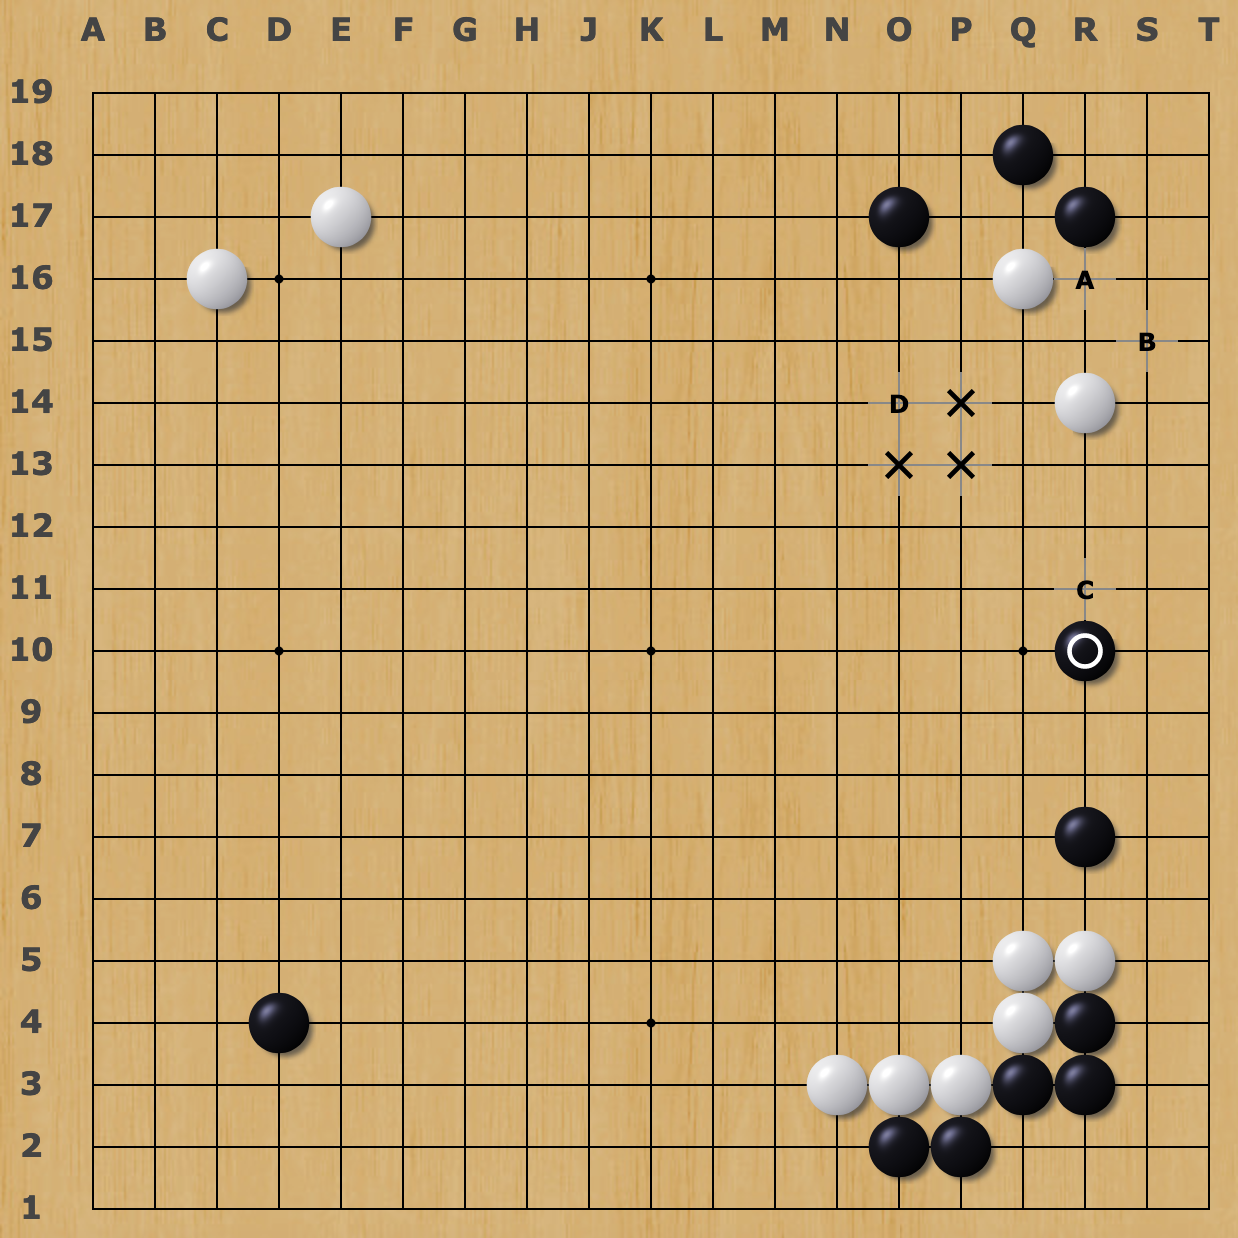
\includegraphics[width=.5\textwidth]{diagram.png}
  \caption{A snapshot of the board state in lines 17--20 of the stream. The (added) marks show the next-move referenants from lines 17--20 as follows: \textbf{A} -- \textit{R16 to get a base}, \textbf{B} -- \textit{S16}, \textbf{C} -- \textit{attach here}, \textbf{D} -- \textit{jump out} (could include moves at any of the \textbf{X}-marked intersections).}
\end{figure}

\noindent Here are some initial observations:
\begin{itemize}
  \item There are at least three different systems of reference used in this short monologue (the three systems, plus one that isn't used here are detailed below). 
  \item Some referring expressions are ambiguous in particular, line 20 \textit{jump out} could refer to a few different possible moves in the same small area.
  \item Referring expressions are often used in conjunction with gesture (in this case, the gestures are made with a mouse cursor).
  \item Many of the same systems of reference are also used to refer to the oponent's previous move. The difference is that previous move reference has the actual move played to draw on as a resource.
  \item Multiple systems of reference can be used at the same time, as in lines 4 and 18.
  \item It's difficult to cleanly decide what speech referrs to a possible move and 
    what asserts something \emph{about} that which is referred. For example, consider 4 (\textit{this attachment that I mentioned before}) and 18 (\textit{play R16 here to get a base}).
\end{itemize}

\noindent Now let's describe the different systems of reference.

\paragraph{absolute coordinates}

As in line 18, one can use the coordinates labelled along the edge of the board
to name a move by the intersection it would occupy.

It's important to note that absolute coordinates are used differently 
in go than in chess.
In chess, the E4 square has a particular identity understood in terms of its
strategic value on the board. 
The name \textit{E4} carries the connotations associated with that identity
and can be used (among experienecd chess players) to refer to that square
even if there is no board in the shared context or the board is not labelled.
In go, this is much less the case. 
In order for \textit{R16} to be meaningful, both the speaker and listener
need to have joint attention on a board that is labelled with numbers and letters.

Part of the reason for this might be that the standard 19x19 go board has many
more intersections than there are chess squares. 

\paragraph{corner-relative coordinates}

\paragraph{demonstratives}

\paragraph{functional descriptors}

\section{Project proposal}

There basic idea is to implement a system that plays go with the user.
It should display a go board and accept voice commands from the user for
where they want play. In the simplest case, the player (or players) can
play both sides or the system can play randomly.

Further features may include:

\begin{itemize}
\item
  More interactive affordances/more natural interaction:

  \begin{itemize}
  \item
    \emph{Oops can I take that move back?}
  \item
    \emph{Sorry I meant \emph{C14} not \emph{C13}.}
  \item
    \emph{Let's start over?}
  \item
    \emph{Can I play as black this time?}
  \item
    Instead of a coordinate command like \emph{B6}:

    \begin{itemize}
    \item
      Player: \emph{I'll \textbf{wedge}.}
    \item
      System: \emph{You want to \textbf{wedge} at \emph{B6}?}
    \item
      Player: \emph{Yes.}
    \end{itemize}
  \end{itemize}
\item
  Integration with variable-strength AI players
\item
  Teaching modules:

  \begin{itemize}
  \item
    basic rules: legal moves, passing
  \item
    how to count points
  \item
    \emph{the rule of ko}
  \item
    basic strategic concepts
  \end{itemize}
\item
  Go terminology: A terminology-teaching routine may be entered through
  a clarification request (Player \emph{What does \textbf{tenuki}
  mean}?)
\item
  Commentary on player moves (System: \emph{That was a somewhat
  \textbf{slow} move. Why don't you try \textbf{cutting} instead?}
  Player: Ok, let's try it.)
\item
  Exploring branching game possibilities
\item
  Playing \emph{tsumego} (go puzzles)
\end{itemize}

\section{Terminology // move descriptors}

Some terms for go moves like \textbf{cut}, \textbf{wedge},
\textbf{kosumi} have straight-forward definitions that depend on the
move's positional relation to nearby stones. Others are more
judgement-based and may need to take the broader board position into
account. Recognizing whether a move can be described as a
\textbf{pincer}, an \textbf{extension}, an \textbf{attachment}, an
\textbf{invasion}, a \textbf{tenuki}, etc. is entirely non-trivial.
Similarly, moves may be described as \textbf{slow}, or as an
\textbf{under-play} or \textbf{over-play}, depending on the move's
strategic value in the overall game. Even certain straight-forward move
descriptors can have less-than-literal interpretations: Technically, two
stones are \textbf{connected} if they are orthogonally adjacent. But
stones that can not be profitably \textbf{cut} by the opponent (for
example because of to surrounding \textbf{influence}) may also be
described as connected.

\section{Data / machine learning}\label{data-machine-learning}

This opens up the possibility for some multi-modal machine learning. Can
we train a language model that can ground some of these go terms in
board positions? It may be possible to scrape an internet corpus that
can be used to train such a model. Go forums (and wikis) often have
special syntax for displaying board positions. A normalized/featurized
version of the board along with the accompanying text may constitute an
interesting data source for training a contextualized language model.

\begin{itemize}
\item
  \href{https://senseis.xmp.net/?HowDiagramsWork}{Sensei's Library}
\item
  \href{https://www.lifein19x19.com/viewtopic.php?f=5\&t=226}{Life in
  19x19}
\item
  Corpora of go commentaries?
\end{itemize}

\hypertarget{possible-experiments}{%
\subsection{Possible experiments}\label{possible-experiments}}

\begin{itemize}
\item
  What strategies are best for teaching go terminology to beginners? How
  do visual demonstrations augment linguistic description?
\item
  How can follow-up questions / clarification requests be accomodated?
\end{itemize}

\section{References}
\printbibliography[heading=none]

\end{document}
